% %!TEX root = ../username.tex
\lstset{
    backgroundcolor=\color{white},
    basicstyle=\footnotesize\ttfamily,
    breaklines=true,
    frame=single,
    captionpos=b,
    numbers=left,
    numberstyle=\tiny\color{gray},
    keywordstyle=\color{blue},
    commentstyle=\color{green},
    stringstyle=\color{red}
}]
\chapter{Development Environment for My Digital Wardrobe App}
\label{chap:Chaptert3}
The development environment for \textit{My Digital Wardrobe} is structured to support efficient cross-platform development, real-time data management, and secure user interactions. This chapter outlines the primary tools, libraries, and configurations used throughout the development process.

Development is conducted on a system running MacOS with 8GB RAM and an Intel i5 processor—a standard setup enabling efficient testing and multitasking. The project’s software stack includes Node.js (version 16.x) and npm (Node Package Manager) for handling dependencies, along with Git for version control. These tools are essential for maintaining compatibility with the project’s core frameworks and libraries.

\section{Core Development Tools}
\label{sec:coredev}
The development of My Digital Wardrobe relies on a combination of  technologies designed to support cross-platform mobile application development, real-time data management, and secure user interactions. These tools were chosen for their robust capabilities, compatibility with the project’s requirements, and their ability to streamline the development process while ensuring scalability and performance. Let’s break down these core tools and libraries, explaining what they are, how they work, and why they are essential for the project.

\subsection{React Native: Building Mobile Apps with Web Technology}
   \textbf{React Native} is is a framework developed by Facebook that allows developers to create \textbf{native mobile applications} (apps that run directly on mobile devices, like those downloaded from the App Store or Google Play) using \textbf{JavaScript}, a popular web programming language.\cite{reactnative} Instead of writing separate code for iOS (using Swift) and Android (using Java or Kotlin), React Native allows the creation of \textbf{cross-platform apps} —one codebase that runs on both platforms. This not only saves time but also reduces development costs. The apps built with React Native look and feel just like apps built with native technologies because React Native uses native components (the building blocks of mobile apps, like buttons, text inputs, and images).
   
\subsection{Expo: Making React Native Easier and Faster}
   \textbf{Expo} is a React native frame work that makes the development process faster and easier, especially for beginners. Think of Expo as a helper toolkit that comes with everything needed to build and test a React Native app. Without Expo, developers would need to set up complex environments for iOS and Android development (like Xcode for iOS or Android Studio for Android), which can be time-consuming and confusing.

   \textbf{Key Features of Expo are:}
\begin{enumerate}
\item \textbf{Pre-Configured Libraries:} Expo comes with many ready-to-use libraries that handle common tasks like accessing the device’s camera, picking images, or sending notifications. This means developers don’t have to build these features from scratch.
\item \textbf{Image Picking: } n this app, Expo’s ImagePicker feature allows users to upload photos of their clothing items directly from their device’s gallery.
\item \textbf{Navigation:} Expo simplifies screen navigation, helping users move smoothly between different parts of the app (like the home screen, wardrobe gallery, and outfit creation pages).
\item \textbf{Easy Testing:} With the Expo Go app, developers can preview their app instantly on a physical device by scanning a QR code—no complex setup required. 
\end{enumerate}
   
\subsection{Firebase: The App’s Brain in the Cloud}
 \textbf{Firebase}: This is a platform developed by Google that provides backend services for mobile and web applications. Think of it as the "brain" of the app that lives on the internet (cloud) and handles all the behind-the-scenes tasks that make the app functional, secure, and fast.

While React Native and Expo handle what the user sees and interacts with (the frontend), Firebase handles the backend—storing data, managing user accounts, and keeping everything running smoothly.

\textbf{Key Firebase Features in our App:}
\begin{enumerate}
    \item \textbf{Firestore (Real-Time Database):}
    \begin{itemize}
        \item Firestore is a cloud-based NoSQL database that stores structured data such as wardrobe items, outfit combinations, and user preferences.
        \item It supports real-time synchronization, ensuring that when a user uploads a new clothing item, it appears instantly in their wardrobe without requiring a manual refresh.
        \item Firestore enables efficient querying and filtering, allowing users to organize and retrieve their wardrobe items based on categories, dates, or other attributes.
    \end{itemize}
    \item \textbf{Firebase Authentication:}
     \begin{itemize}
        \item Authentication is crucial for protecting user data and ensuring privacy.This feature manages user sign-up, login, and secure access.
        \item It ensures that each user has their private wardrobe that only they can access, using secure methods like email/password authentication or third-party logins (e.g., Google, Facebook).
    \end{itemize}
    \item \textbf{Firebase Storage:}
     \begin{itemize}
        \item Firebase Storage is used for securely storing media files, specifically images of clothing items uploaded by users.
        \item Each image is stored securely and linked to the user’s profile as a file, and a corresponding download URL is generated, which is then linked to the item’s metadata in Firestore. The app retrieves these images whenever needed, displaying them in the user’s digital wardrobe.
        \item Firebase ensures that images are accessible across multiple devices, so users can manage their wardrobe anywhere, anytime.
    \end{itemize} 
\end{enumerate}


\subsection{Git and GitHub: Keeping Track of Changes and Collaboration}
   \textbf{Git} is a free and opensource version control system. Think of it as a "save game" feature for development. If something breaks or a mistake is made, Git allows developers to go back to a previous version without starting over. \textbf{Github} is an online platform where Git-managed projects are stored. It allows multiple developers to work on the same project simultaneously , tracking who made what changes and merging everyone’s work easily.  Together they provide robust version control and repository management, allowing easy collaboration and efficient tracking of changes.
   
\textbf{How Git and GitHub Were Used in Our Project}
\begin{itemize}
\item \textbf{Version Control :} Every change made during development—whether adding new features or fixing bugs—is recorded. This makes it easy to track progress and revert to earlier versions if needed.
\item \textbf{Collaboration :} Although this project is independently developed, GitHub would enable collaboration by letting multiple developers contribute without overwriting each other’s work.
\item \textbf{Branching :} GitHub supports creating branches—independent lines of development. For example, one branch could be used for developing the image upload feature, while another focuses on user authentication. These branches can later be merged into the main project once they’re tested and stable.
\item \textbf{Backup :} GitHub acts as a cloud backup for the project, ensuring that the latest version of the code is safe and accessible from any device.
\end{itemize}

\section{Comparison of React and React Native}
Although this project exclusively uses \textbf{React Native}, understanding its differences from React clarifies its selection as the framework of choice. While both frameworks share a \textbf{JavaScript} foundation and adopt a \textbf{component-based architecture}, they serve fundamentally different purposes in software development. The comparison in Table~\ref{tab:react-comparison} outlines the key distinctions between React and React Native, providing context for why React Native was selected for the development of My Digital Wardrobe.


\begin{table}[h]
    \centering
    \begin{tabular}{|p{3.5cm}|p{4.5cm}|p{4.5cm}|}
        \hline
        \textbf{Aspect} & \textbf{React} & \textbf{React Native} \\
        \hline
        Purpose & Primarily for building web applications. & Designed for creating native mobile applications for iOS and Android. \\
        \hline
        Rendering & Renders components into the DOM using HTML and CSS. & Renders components into native UI elements using platform-specific APIs. \\
        \hline
        Components & Utilizes HTML-like components (e.g., \texttt{<div>}, \texttt{<span>}). & Uses platform-specific components (e.g., \texttt{<View>}, \texttt{<Text>}). \\
        \hline
        Styling & Leverages CSS or pre-processors like SCSS for styling. & Utilizes \texttt{StyleSheet} for styling, similar to CSS but tailored for mobile. \\
        \hline
        Cross-Platform & Limited to web platforms. & Supports cross-platform development for iOS and Android. \\
        \hline
        Performance & Relies on browser rendering, which may impact performance for complex UI. & Renders native elements, leading to better performance for mobile apps. \\
        \hline
        Libraries and Ecosystem & Rich ecosystem of libraries for web development (e.g., React Router). & Includes libraries like Expo for streamlined mobile app development. \\
        \hline
        Development Tools & Uses browser-based debugging tools and extensions like React DevTools. & Provides platform-specific debugging tools (e.g., Android Studio, Xcode). \\
        \hline
    \end{tabular}
    \caption{Comparison of React and React Native}
    \label{tab:react-comparison}
\end{table}

As shown in Table~\ref{tab:react-comparison}, \textbf{React} is primarily used for building web applications. It renders components using web technologies such as HTML, CSS, and JavaScript, which are interpreted by web browsers. While React excels at creating dynamic and responsive web interfaces, it is limited to the web platform and cannot leverage native device features without additional tools or frameworks. This limitation makes React less suitable for applications requiring close integration with mobile device capabilities, such as camera access or gesture-based navigation .

Conversely, \textbf{React Native} was designed specifically for creating \textbf{native mobile applications} for \textbf{iOS} and \textbf{Android} platforms. Instead of rendering components to a web browser’s Document Object Model \textbf{(DOM)}, React Native renders them into \textbf{native UI components} using platform-specific APIs. This approach allows applications built with React Native to achieve \textbf{near-native performance}, offering users an easy and responsive experience that is indistinguishable from fully native apps developed with platform-specific languages like Swift for iOS or Kotlin for Android \cite{reactnative}.

Moreover, React Native supports a \textbf{component-based structure}, which allows for the creation of reusable, interactive user interfaces. This modularity is essential for My Digital Wardrobe, where features such as wardrobe browsing, image uploading, and outfit creation can be developed as independent components. Such an approach simplifies maintenance, enhances scalability, and allows for faster implementation of new features, aligning perfectly with the project’s requirements for flexibility and user-centric design.

Another critical consideration in selecting React Native is its \textbf{performance advantage} over web-based mobile frameworks. React Native applications do not rely on browser rendering, which can introduce performance bottlenecks in complex user interfaces. Instead, React Native translates UI components into native code, ensuring that animations, transitions, and interactions are smooth and responsive. This capability is particularly important for My Digital Wardrobe, where users frequently interact with high-resolution images and expect real-time updates when creating and managing outfits.

Furthermore, React Native boasts a robust ecosystem supported by an active developer community\cite{reactnative}. The availability of well-maintained libraries, tools, and documentation accelerates development and minimizes potential challenges. This ecosystem is further enhanced by the full integration of Expo, which simplifies access to native device features and streamlines testing and deployment processes. While the details of Expo, Firebase, and version control practices have been discussed in the previous Section \ref{sec:coredev}, it is important to note that React Native’s compatibility with these tools forms the backbone of the app's development workflow.

\begin{figure}[h]
    \centering
    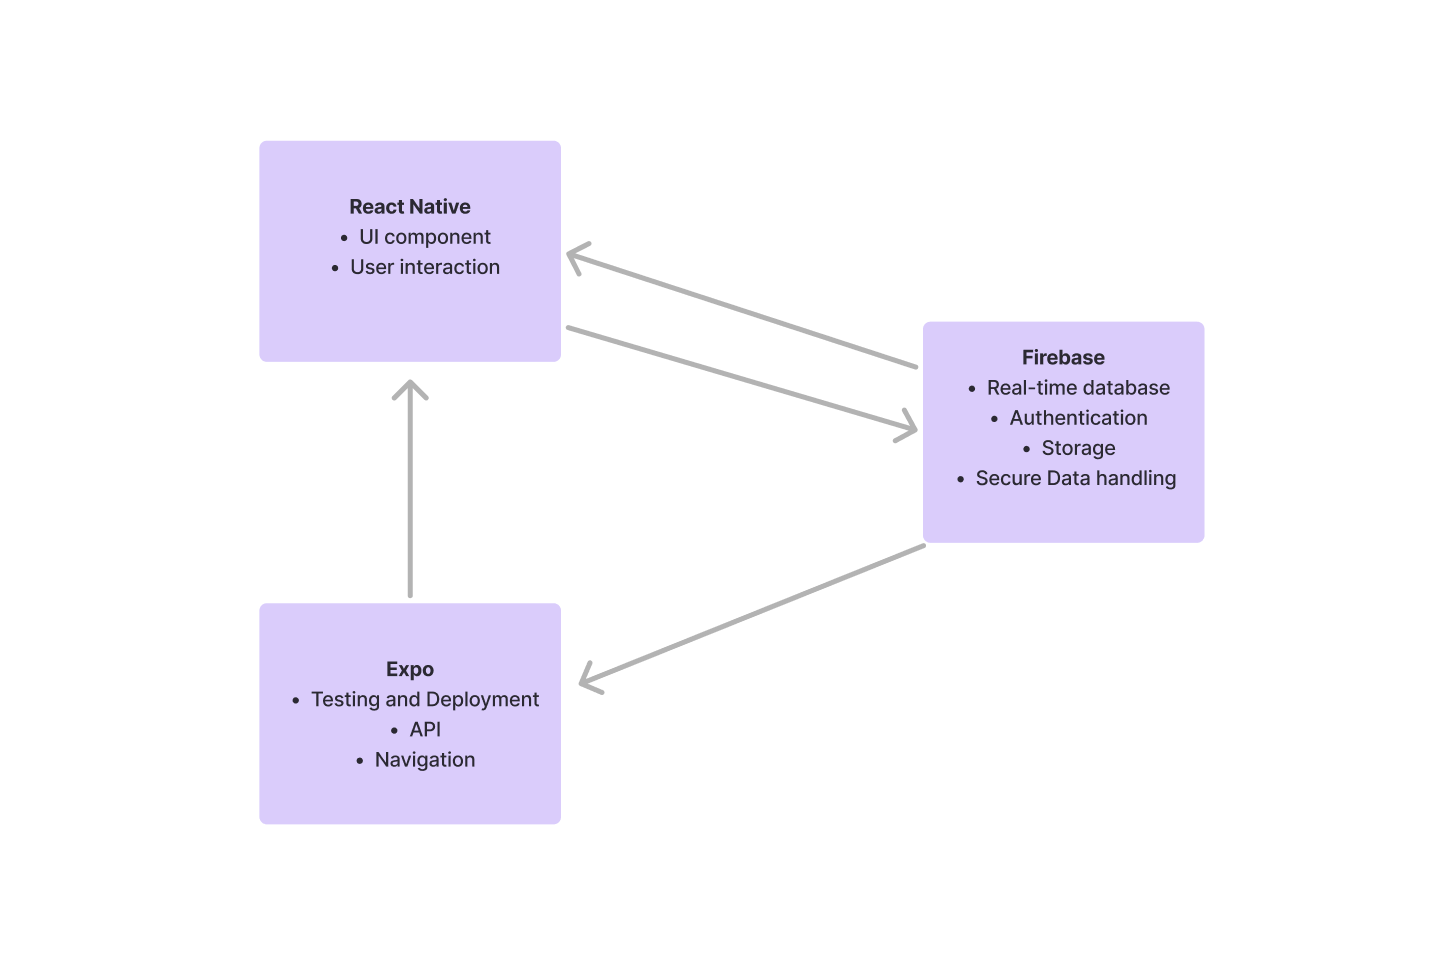
\includegraphics[width=1.2\linewidth]{exampleis-master/figures/Chapt3.3.png}
    \caption{The relationships between React Native, Expo, and Firebase, along with their respective roles in the app.}
    \label{fig:integration1}
\end{figure}

As shown in Figure \ref{fig:integration1}, React Native forms the core UI, providing a consistent user experience. It integrates with Expo for device-specific features like image selection and navigation, while Firebase manages real-time data, user authentication, and media storage. This streamlined workflow ensures secure, responsive, and cross-platform functionality.


\section{Supporting Libraries and Dependencies}
Several supporting libraries are included to handle essential functionalities and enhance the app’s user experience:

\begin{itemize}
     \item \textbf{Expo Router}: 
     The \texttt{expo-router} library plays a crucial role in managing navigation within the application. It enables structured and dynamic transitions between screens, ensuring that users can easily move through different parts of the app. For instance, we can see in Chapter \ref{chap:Chaptert5} , Listing \ref{lst:index} the navigation between the \texttt{LoginScreen} and \texttt{HomeScreen} is dynamically managed based on the user’s authentication status. This approach allows the app to direct users to appropriate screens without manual intervention, maintaining a coherent flow throughout the application. The use of \texttt{expo-router} eliminates the complexity of handling navigation manually, allowing for organized routing that responds automatically to user interactions and authentication changes.

    \item \textbf{Firebase SDK}: The \textbf{Firebase Software Development Kit (SDK)} is a core dependency, providing direct access to essential services discussed in Section \ref{sec:coredev} like Firestore, Authentication, and Storage services.
    The following code snippet in Listing \ref{lst:firebase_setup} demonstrates the Firebase setup used in the project. It outlines the configuration required to initialize Firestore, Authentication, and Storage services, ensuring proper data management and secure user access across the app\cite{firebasecookbook}.

\end{itemize}
\begin{lstlisting}[caption={Firebase Setup}, label={lst:firebase_setup}, numbers=left,stepnumber=1, numberstyle=\tiny\color{gray}]
import { initializeApp } from "firebase/app";
import { getFirestore, getAuth, initializeAuth, getStorage } from "firebase";
import AsyncStorage from "@react-native-async-storage/async-storage";
const firebaseConfig = {
    apiKey: "YOUR_API_KEY",
    authDomain: "YOUR_PROJECT.firebaseapp.com",
    projectId: "YOUR_PROJECT",
    storageBucket: "YOUR_PROJECT.appspot.com",
    messagingSenderId: "YOUR_SENDER_ID",
    appId: "YOUR_APP_ID"
};
const app = initializeApp(firebaseConfig);
export const db = getFirestore(app);
export const auth = initializeAuth(app, { persistence: getReactNativePersistence(AsyncStorage) });
export const storage = getStorage(app);
\end{lstlisting}


Following the Firebase setup shown in Listing \ref{lst:firebase_setup}, it is essential to break down the code to provide a clear understanding of how Firebase services are integrated into the application. Each part of the code plays a crucial role in ensuring that user data, authentication, and media storage are managed effectively.

The first three lines import the necessary modules required to access Firebase services. The \textbf{initializeApp} function from  \textbf{Line 15} is used to initialize the Firebase application with the configuration settings provided via lines  \textbf{Lines6-12}. The functions \textbf{getFirestore}, \textbf{getAuth}, \textbf{initializeAuth}, and \textbf{getStorage} provide access to Firebase's key services. \textbf{AsyncStorage} is imported to ensure user authentication sessions persist even after the app is closed, enhancing user convenience.

 \textbf{Line6-13} it defines the Firebase configuration object, which contains unique identifiers and keys that connect the app to the specific Firebase project. Each key serves a distinct purpose:
\begin{itemize}
\item \textbf{apiKey} authenticates requests from the app to Firebase services.
\item \textbf{authDomain} specifies the domain used for authentication processes.
\item \textbf{projectId} identifies the Firebase project associated with the app.
\item \textbf{storageBucket} refers to the cloud storage location where user images are stored.
\item \textbf{messagingSenderId and appId} helps manage notifications and application identification.
\end{itemize}

In the final part of the setup, (\textbf{lines 15-18})Firebase services are initialized:

\begin{itemize}
\item \textbf{initializeApp(firebaseConfig)} activates Firebase within the application using the previously defined configuration.
\item \textbf {getFirestore(app)} initializes Firestore, which stores user wardrobe data, including item details and metadata.
\item \textbf {initializeAuth(app, {persistence: getReactNativePersistence(AsyncStorage) })} initializes Firebase Authentication. The persistence setting ensures that the user's login session is remembered, so they remain logged in even after closing the app.
\item \textbf {getStorage(app)} sets up Firebase Storage, which securely stores user-uploaded clothing images. These images are linked to user profiles and can be accessed across devices.
\end{itemize}

\section{Development Configurations}
To ensure consistency and compatibility across different development environments, specific configurations are established. These configurations not only support efficient development but also safeguard sensitive information and optimize the app's performance across multiple platforms.

\textbf{The Node Package Manager (npm)} plays a central role in managing the application’s dependencies. Node.js, in version 16.x, was selected due to its compatibility with the core libraries used in the project. The \texttt{package.json} file outlines all dependencies along with their specific versions. This setup ensures that developers working on the project can initialize identical environments, preventing issues related to mismatched library versions. By maintaining consistency in the development environment, the risk of integration errors is minimized, and collaborative work becomes more efficient \cite{nodeessentials} \cite{nodecompleteguide}.
Managing sensitive information, such as Firebase API keys and configuration settings, was addressed through the use of environment variables. These variables are stored in \texttt{.env} files, which are excluded from version control to prevent unauthorized access. This approach ensures that sensitive data remains secure while still being accessible during development. By separating configuration data from the core codebase, the application remains flexible, allowing for easy modifications to environment-specific settings without altering the main code.

Another critical aspect of the development configuration involves platform-specific testing and debugging. The \textbf{Expo CLI} provides tools for testing the application across various devices and platforms. Commands like \texttt{expo start} enable real-time testing on both physical devices and emulators, facilitating the identification and resolution of platform-specific issues. This testing strategy is particularly important for features such as image uploads and gesture-based navigation, which can behave differently on iOS and Android. Ensuring compatibility across these platforms improves the reliability of the application and provides a consistent user experience.


\section{Summary of Development Tools}
The development tools and configurations described in this chapter form the backbone of My Digital Wardrobe. The use of \textbf{ React Native} and \textbf{Expo} ensures a uniform user interface and responsive performance across iOS and Android devices \cite{reactnative}. \textbf{Firebase} provides robust backend support, managing data storage, authentication, and media handling in a secure and scalable manner. Additionally, the development configurations, including consistent package management, secure handling of environment variables, and comprehensive platform testing, contribute to a stable and adaptable development process\cite{reactfirebase} \cite{firebasecookbook}.

With this structured environment in place, the subsequent chapter, Chapter \ref{chap:Chapter4} will provide an in-depth exploration of the system architecture of \textit{ My Digital Wardrobe}. It will examine how the selected tools and configurations support the application's core components, including navigation flows, real-time data management, and media storage integration. The discussion will highlight how each element contributes to the overall performance, scalability, and user experience of the application.


